\section{论文概览}

\subsection{论文要回答的问题}

这篇论文研究的不是“视频扩散模型如何生成更清晰、更逼真的视频”，而是一个更机制化的问题：当视频扩散模型在迷宫、物体移动、图形补全、旋转、目标定位等任务中表现出推理能力时，这种推理究竟在模型内部沿什么维度展开。

已有直觉常把视频推理理解为 Chain-of-Frames (CoF)：模型像看电影一样，沿着帧的时间顺序一帧一帧推进推理。本文反驳这一假设，提出 Chain-of-Steps (CoS)：扩散视频模型的主要推理轴不是 frame，而是 diffusion denoising step。也就是说，模型不是先想完第 1 帧再想第 2 帧，而是在每一个去噪步骤中同时更新整段视频，并随着去噪过程逐渐精炼候选假设。

\subsection{一句话总结}

Demystifying Video Reasoning 的核心发现是：视频扩散模型的推理主要沿扩散去噪步骤展开；早期步骤进行多候选探索，中期步骤剪枝并巩固结论，后期步骤整合细节，而在单个去噪步骤内部，DiT 层又呈现从感知到目标聚焦再到推理整合的功能分工。

\subsection{为什么这篇论文难}

这篇论文难在它跨越三个层次：

\begin{itemize}
    \item 扩散生成层：需要理解 noise、latent、clean estimate、velocity field、scheduler、VAE decoder、CFG 等概念。
    \item 推理机制层：需要区分 CoF 与 CoS，理解多路径探索、叠加式探索、噪声扰动和信息传播。
    \item 神经网络内部层：需要理解 DiT layer、hidden state、forward hook、token reshape、activation energy 和 latent swapping。
\end{itemize}

因此阅读时不能只看最终视频结果，而要同时看三个坐标轴：视频帧轴、扩散步骤轴和 Transformer 层深度轴。本文的贡献正是把这些轴拆开分析，说明哪一个轴更接近“推理发生的位置”。

\subsection{主要贡献}

\begin{enumerate}
    \item 提出 Chain-of-Steps，挑战“视频推理沿帧顺序展开”的 Chain-of-Frames 假设。
    \item 通过逐步解码每个 diffusion step 的 clean latent estimate，观察到多路径探索和叠加式探索。
    \item 通过 step-wise 与 frame-wise 噪声扰动证明：破坏特定扩散步骤比破坏单个视频帧更严重。
    \item 发现类似 LLM 的突现推理行为，包括工作记忆、自我修正和先感知后行动。
    \item 对 Diffusion Transformer 做逐层机制分析，发现早层偏感知，中层承载关键推理，后层负责整合。
    \item 基于 CoS 机制提出无训练的 inference-time latent ensemble，作为利用多路径探索提升推理能力的概念验证。
\end{enumerate}

\subsection{Figure 1 的核心直觉}

Figure~\ref{fig:figure1} 是全文最重要的图之一。它用迷宫任务展示：早期 diffusion steps 中，模型并不会立即给出一条明确路径，而是会在 latent 中同时保留多条候选路径；中期步骤逐渐压制错误路径；后期步骤收敛到唯一最终答案。

\begin{figure}[H]
    \centering
    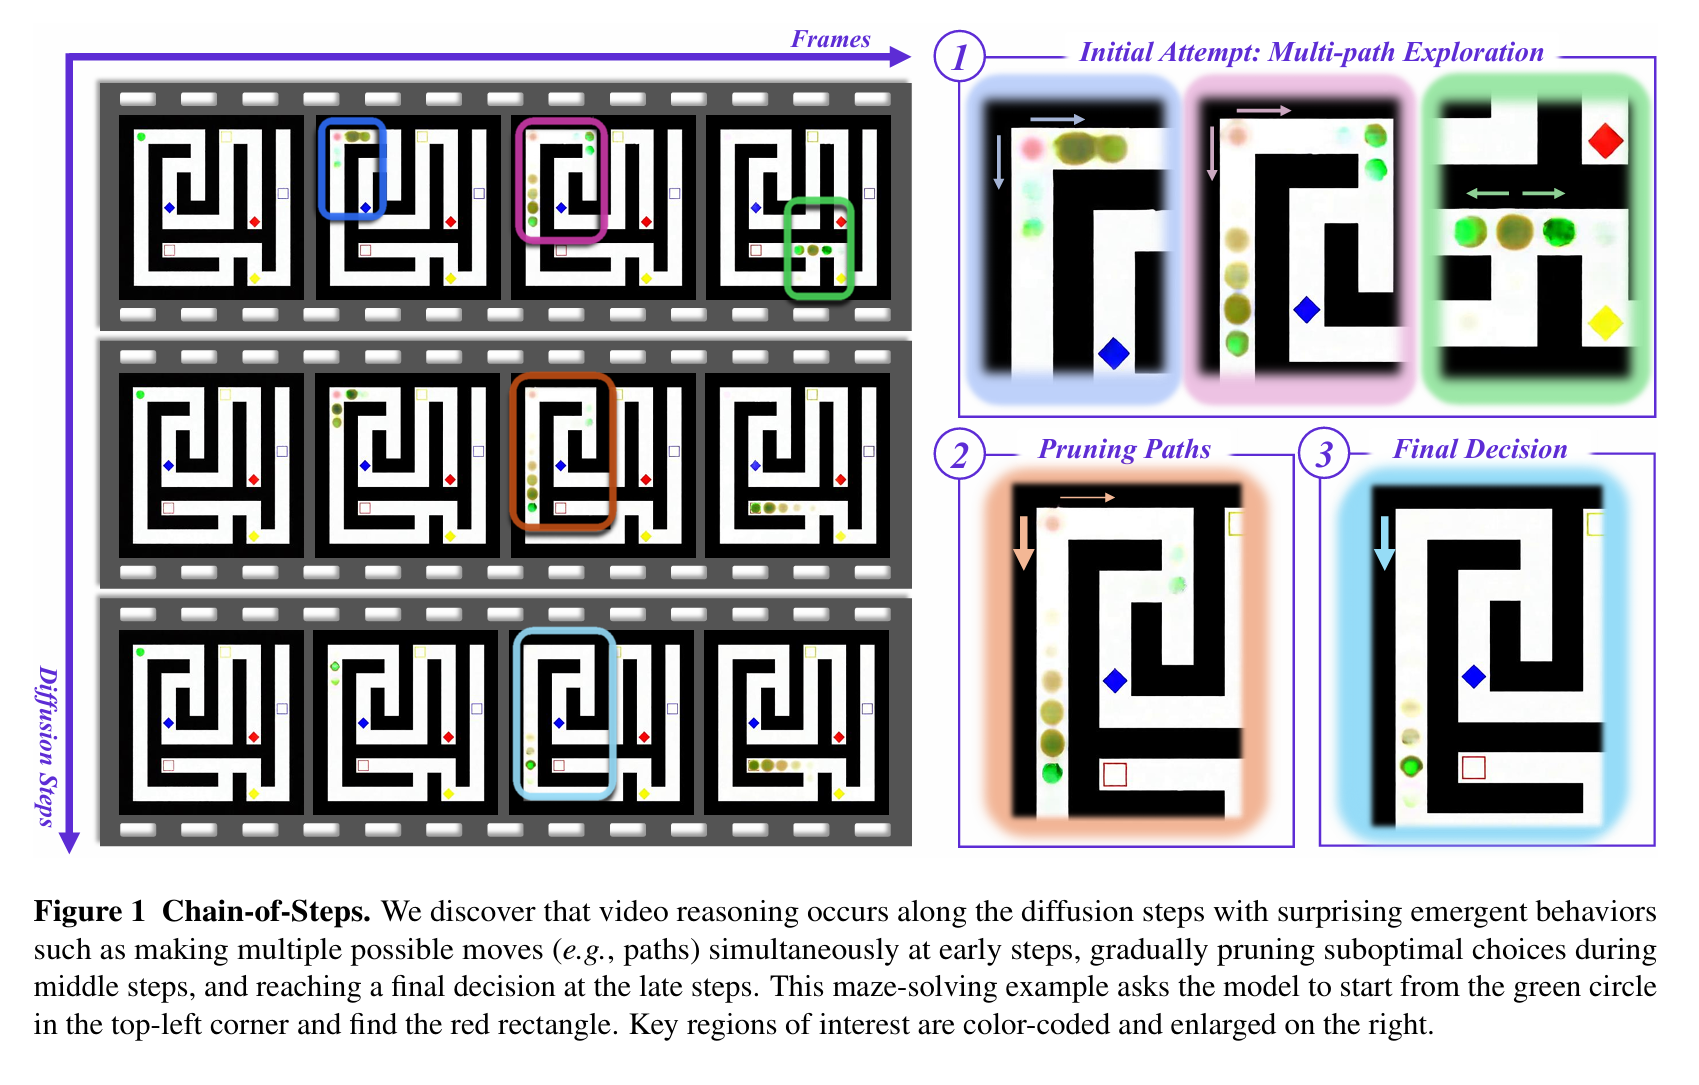
\includegraphics[width=0.96\textwidth]{figures/figure1.png}
    \caption{Chain-of-Steps 的核心示意：扩散模型先多路径探索，再剪枝，最后形成最终决策。}
    \label{fig:figure1}
\end{figure}

这张图最重要的读法是：横轴是 video frames，纵轴是 diffusion steps。真正显著的推理变化主要发生在纵向，即同一帧随着 diffusion step 推进而从多候选变成单一解。这正是 CoS 支持证据，而不是 CoF 支持证据。
